\chapter{Projekt  Breakthrough }
\label{projekt.breakthrough}

\tikzset{pgfornamentstyle/.style={line width=0.05pt}}
\def\wP#1#2{
    \filldraw[fill=white,draw=black] (#1,#2) circle (0.4);
    \node[very thin] at (#1,#2) {\pgfornament[width = 0.46cm,color = black]{12}};
}
\def\wPn#1#2#3{
  \wP#1#2
  \node[circle, fill=white, inner sep = 0.5pt] at (#1,#2) {#3};
}
\def\bP#1#2{
    \filldraw[fill=black,draw=black] (#1,#2) circle (0.4);
    \node[very thin] at (#1,#2) {\pgfornament[width = 0.46cm,color = white]{4}};
}
\def\bPn#1#2#3{
  \bP#1#2
  \node[circle, fill=black, color=white, inner sep = 0.5pt] at (#1,#2) {#3};
}
\def\boardBg{
  \fill[fill=teal!10!white] (-0.5,-0.5) rectangle (7.5,7.5);
}
\def\boardGrid{
  \draw[shift={(-0.5,-0.5)}] (0,0) grid (8,8);
  \foreach\c[count=\i] in {a,b,c,d,e,f,g,h} \node[below = 0.4] at (\i-1,0) {\c\strut};
  \foreach\i in {1,2,...,8} \node at (-0.9,\i-1) {\i};
}
\def\wPs#1{
    \foreach \x in {#1} {      
      \expandafter\wP\x
    }
}
\def\bPs#1{
    \foreach \x in {#1} {      
      \expandafter\bP\x
    }
}
\def\wC#1{\raisebox{-0.4ex}{\LARGE\libcirc{#1}}}
\def\bC#1{{\LARGE\libcircblk{#1}}}


V nasledujúcich častiach ti ukážem niekoľko ďalších vecí v C++, ktoré je ale najlepšie
vidieť na trochu väčších programoch. Začneme preto s projektom, ktorý nás bude sprevádzať 
dlhší čas: našim cieľom bude napísať program, ktorý hrá hru \btr\footnote{Pravidlá som prevzal z 
\href[pdfnewwindow=true]{https://trmph.com/bin/Basic_Introduction_to_Breakthrough.pdf}{\nolinkurl{https://trmph.com/bin/Basic_Introduction_to_Breakthrough.pdf}}}.
Hru \btr vymyslel r. 2000 Dan Troyka. Jej výhodou je, že má veľmi jednoduché pravidlá
(v porovnaní napr. so šachom),
takže sa ľahko programuje, ale zároveň vôbec nie je jednoduchá na hranie. 
Hrá sa na šachovnici $8 \times 8$. Hrajú dvaja hráči (biely a čierny) a na začiatku
má každý hráč 16 kameňov umiestnených takto:\\
\label{pg:breaktru:def}


\centerline{
%\tikzset{external/force remake}
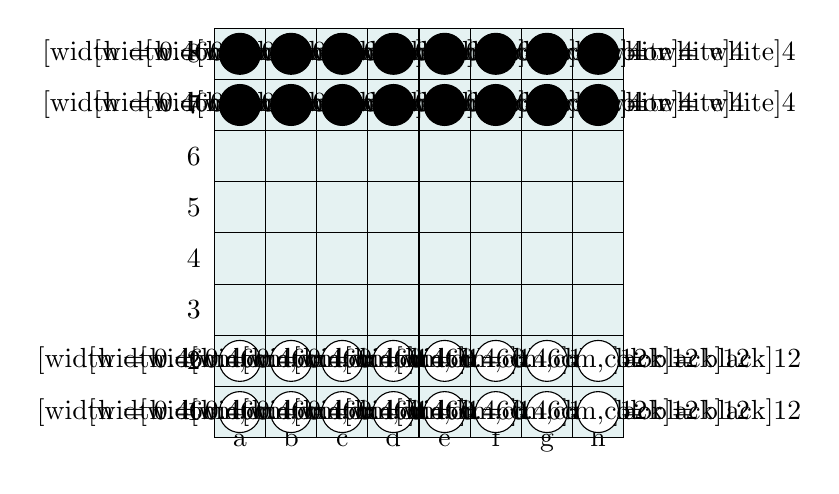
\begin{tikzpicture}[scale=0.65]
  \boardBg
  \boardGrid
  \wPs{00,10,20,30,40,50,60,70,01,11,21,31,41,51,61,71}
  \bPs{07,17,27,37,47,57,67,77,06,16,26,36,46,56,66,76}
\end{tikzpicture}
}

Hráči sa striedajú na ťahoch (začína biely), pričom v každom ťahu si hráč
vyberie nejaký svoj kameň a pohne ním. Cieľom je dostať niektorý svoj kameň na opačný
koniec šachovnice. Komu sa to podarí prvému, vyhrá (ak hráč príde o všetky
svoje kamene, automaticky prehral). Hráč môže pohnúť svoj kameň o jedno políčko
rovno alebo šikmo, ak je cieľové políčko voľné. Navyše, ak je na cieľovom
políčku súperov kameň, hráč ho môže vyhodiť, ale iba šikmo (ako pešiak v
šachu).




\begin{minipage}[t]{0.5\textwidth}\vspace*{0cm}
\centerline{
%\tikzset{external/force remake}
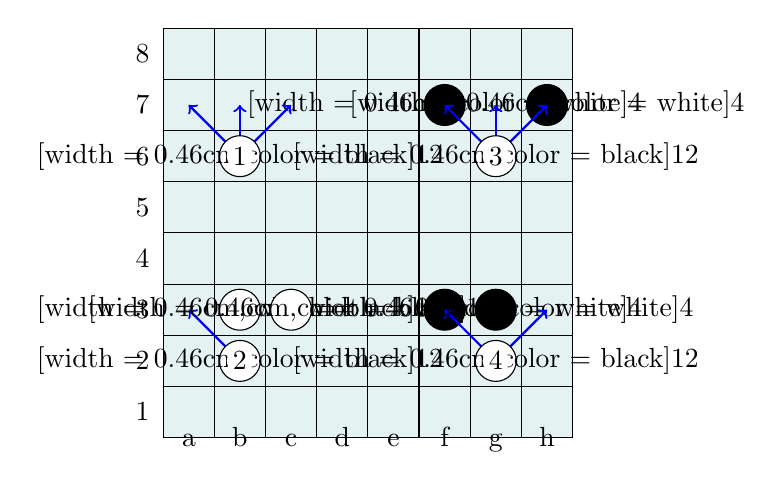
\begin{tikzpicture}[scale=0.65]
  \boardBg
  \boardGrid
  \bPs{56,76}
  \bPs{52,62}
  \foreach \y in {5,6,7} 
  \draw[blue,thick,->](6,5)--(\y,6);

  \foreach \y in {0,1,2} 
  \draw[blue,thick,->](1,5)--(\y,6);
  
  \draw[blue,thick,->](1,1)--(0,2);
  
  \draw[blue,thick,->](6,1)--(5,2);
  \draw[blue,thick,->](6,1)--(7,2);
  
  \wPn151
  \wPn112
  \wPs{12,22}
  \wPn653
  \wPn614

\end{tikzpicture}
}
\end{minipage}
\begin{minipage}[t]{0.5\textwidth}\vspace*{0cm}
Príklad pravidiel: biely kameň \wC1 môže ísť z b6 na a7, b7, alebo c7, lebo všetky sú voľné.
Biely kameň \wC2 z b2 môže ísť iba na a3, lebo b3 a c3 sú blokované.
Biely kameň \wC3 z g6 môže ísť na f7, g7, alebo h7, pričom ak pôjde na f7 alebo h7
tak zoberie súperov kameň. Napokon kameň \wC4 z g2 môže buď zobrať súpera na f3, alebo prejsť
na h3, ale nemôže ísť na g3.
\end{minipage}




